% Chapter APNA Overlay

\chapter{APNA inside SCION} % Main chapter title

\label{apna_overlay}

\section{Main Idea}

The main idea behind this approach is to encapsulate APNA packet as a payload to the SCION packet. 

First of all why would someone do this? The answer would be it requires least amount of modification in the current infrastructure which makes its deployment very easy. Since it is not dependent on other SCION infrastructure, this loose coupling with other components helps a lot in the development of APNA protocol.

Initially when the SCION packet is constructed L4 address is set to random IPv4/IPv6 address until the packet reaches the last hop border router. At the last hop border router it looks at APNA packet and decrypts the destination EphID to find out which dispatcher it needs to forward this packet. It also replaces the random L4 destination address with recently decoded address, so that dispatcher does not have perform the same translation.

\section{Modification in the current infrastructure}
\subsection{Border Router}
Border Routers needs to connect to APNA Management Service for the following reasons:
\begin{itemize}
    \item \textbf{MAC Verification:} In order to perform MAC verification for the outgoing packet Border Router at source AS would need the key with which the packet was signed. But since that key is only registered with the APNA Management Service. Border Routers needs to contact the Key Management Service (Sec. \ref{kms}) for that key. Since contacting APNA Management Service every time a packet comes in could be expensive. So it implements a small cache of replies which it received from the Key Management Service for fast packet processing. Currently it's a very simple cache based on First in First Out (FIFO) replacement policy, but it would be interesting to investigate other caching policies like Least Recently Used (LRU) etc.
    \item \textbf{IP address from HID:} In order to find right dispatcher for inter-domain packet forwarding, destination border router needs to decrypt the destination EphID and get the host identifier. But dispatcher only understands IP address, so border router performs the translation from Host Identifier to IP address and updates the SCION packet L4 destination address. With the help of identity management service (Sec. \ref{ims}) it performs the translation from host identity to IP address. It also maintains a cache of this mapping for fast packet processing like MAC verification.
\end{itemize}
Note that the above modifications are only required at the source and destination border router. Rest of the border routers can still run the old version of border router which does not support APNA Protocol.

\subsection{SNET}
Since we no longer wants to use IP address for our communication the main networking library needs to be modified to accommodate that request. In order to accomplish this \texttt{snet.ListenSCION()} and \texttt{snet.DialSCION()} needs a accept a new network string parameter "\texttt{apna}". Before this it only supported "\texttt{udp4}". Accordingly the \texttt{read} and \texttt{write} methods provided by interface \texttt{snet.Conn} also needs to be modified as they deal with creating and parsing the SCION packet.

\section{Data Communication}
In order to communicate on the network, a host needs to initialize the networking context with snet and register its IP address with dispatcher. Once a host is successfully registered with dispatcher it can contact the APNA Management Service to issue an Session EphID to the host. Then the host will contact the DNS service to obtain the EphID of the server that it wants to talk to. After that host could initialize the APNA handshake by creating the first APNA packet. When the SCION packet is constructed L4 src and dst address are filled with random bytes and in the payload you can find the APNA packet. When the border router at the src AS gets that packet. It performs some local processing to convert payload back to APNA Packet and perform MAC verification before forwarding it to the neighbouring BR mentioned in path information.

\subsection{Data Forwarding}
A border router in the source AS ensures that only packets from authenticated hosts and authorized EphIDs leave the AS; and a border router in the destination AS forwards the packets to correct dispatcher based on the destination EphID. Transit ASes do not perform additional operations and simply forward the packets to the next AS mentioned in the SCION header path information. In order to achieve high performance data forwarding, only symmetric cryptographic operations are used.

Communication end-points are specified as ISD-AS:EphID tuples. For inter-domain forwarding, border routers use only ISD-AS to forward packets. Specifically, for external packets entering the AS, a border router checks whether the packet has arrived at the destination AS (Figure \ref{fig:overlay_dst}). If not, the packet is forwarded to the next AS mentioned in the Path Information in the SCION packet (Line 9). At the destination AS, the border router performs the following conditions: 1) the destination EphID ($EphID_{d}$) is valid, i.e., has not expired (Line 4).

If all the conditions are satisfied, then the border router tries to resolve IP address from $HID_{d}$ with the help of APNA Management Service. First border check its own cache of IP address from HID, if the HID is not present in its cache it would sent a host resolution query to the APNA management service. If the APNA Management Service replies with $ErrHostNotPresent$ it drops the packet and abort. If it replies with $ErrorOK$, then border router forwards the packet to the dispatcher by setting the destination IP address with the reply sent from Management Service. Then the dispatcher forwards the packet according to the host mapping it has depending upon the host which registered with it in the first step.

For outgoing packets, a border router forwards the packet to a neighboring AS only if all the following conditions are satisfied: 1) the source EphID ($EphID_{s}$) is valid i.e., has not expired (Line 3 in the \ref{fig:overlay_src}) 2) the MAC in the packet is correct (Line 6).

To verify the MAC in the packet, a border router retrieves the shared key ($k_{HA}$) between the source host and the AS by searching the host information database ($host\_info$). Entries in this database are populated with the help of APNA Management Service using its Key Management Service (\ref{kms})

\begin{figure}[th!!]
\centering
\hspace*{2cm}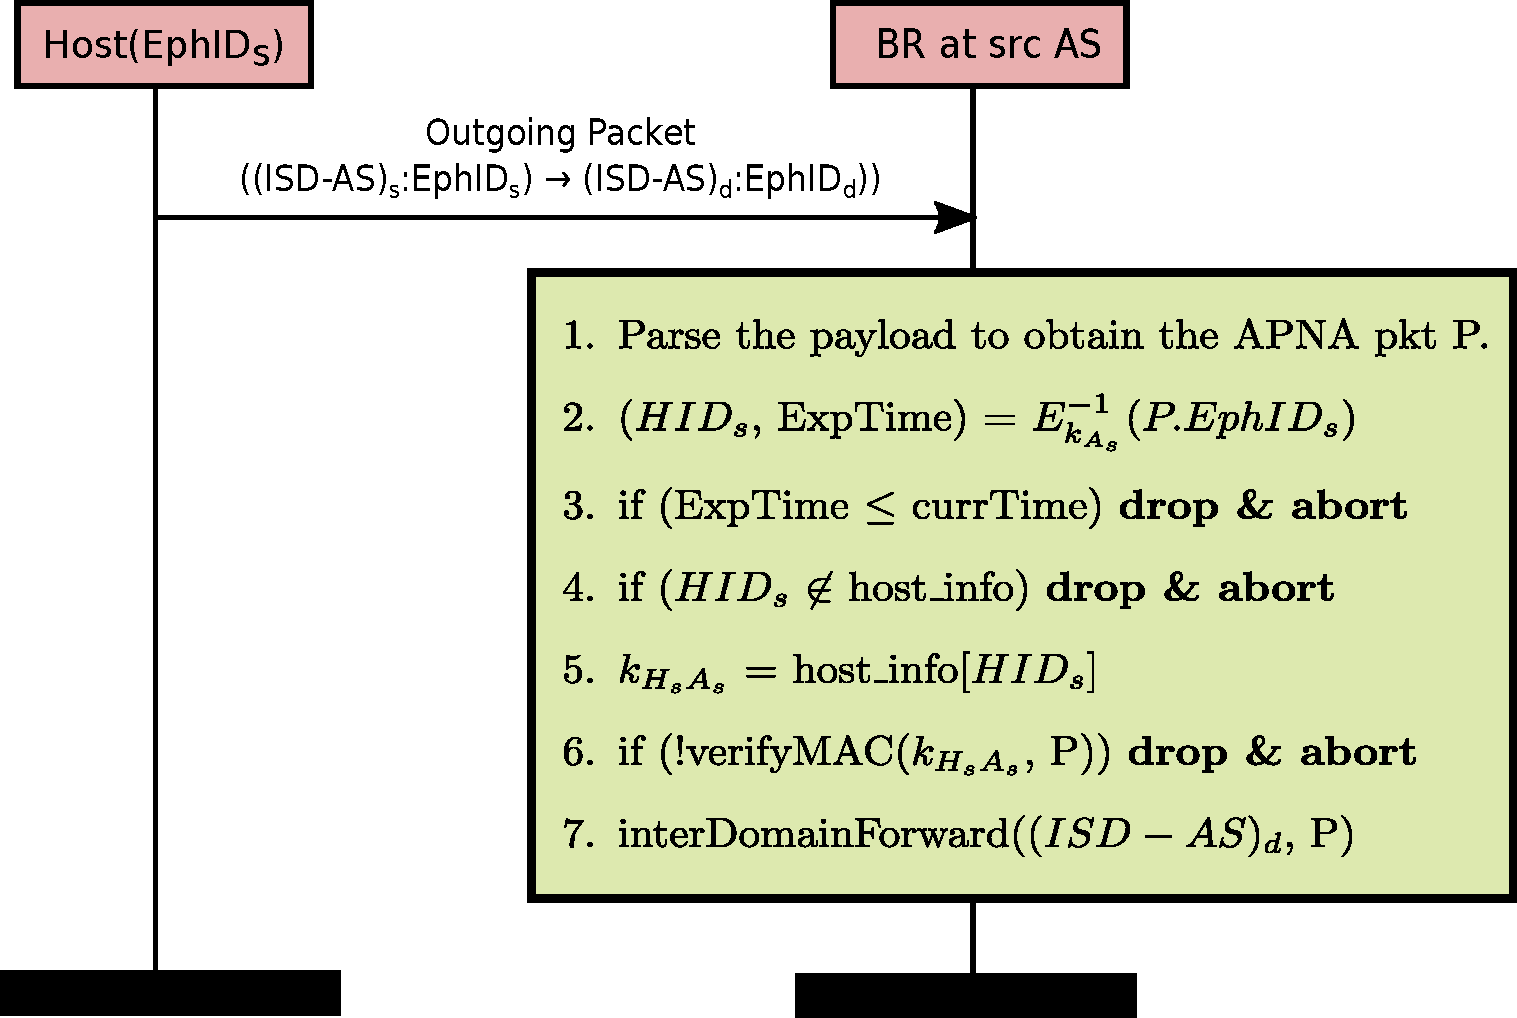
\includegraphics[scale=0.5]{Figures/overlay_src.pdf}
\decoRule
\caption[Apna Overlay Outgoing Packet]{Outgoing Packet}
\label{fig:overlay_src}
\end{figure}

\begin{figure}[th!!]
\centering
\hspace*{2cm}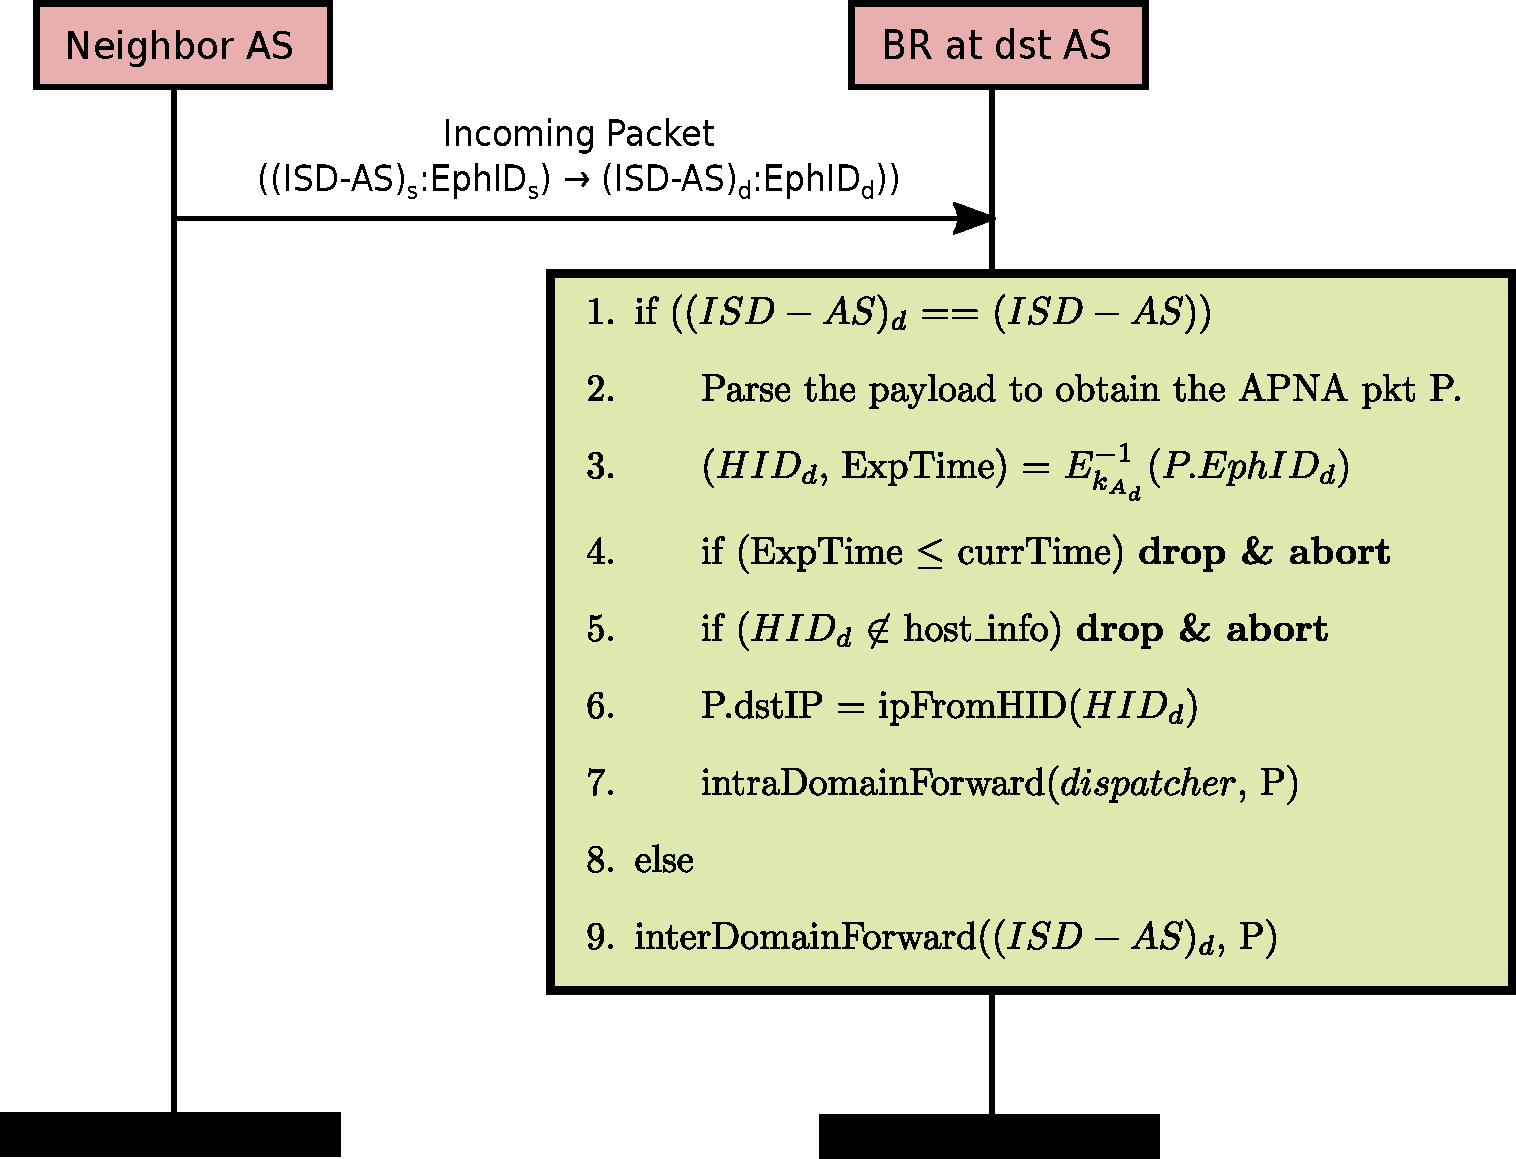
\includegraphics[scale=0.5]{Figures/overlay_dst.pdf}
\decoRule
\caption[Apna Overlay Incoming Packet]{Incoming Packet}
\label{fig:overlay_dst}
\end{figure}
